\newpage
\section{Report 03: Building model \textit{Drosophila}}

\subsection*{2021-04-01}

\subsection{Introduction}
Before carrying out the experiments, model \textit{Drosophila} should be prepared using molecular and genetic methods. In this session, we discussed about the details of constructing the model \textit{Drosophila} needed in next experiments.


\subsection{Results \& Discussion}
Since the two models are based on different mechanisms, we will talk about how these models work and how to construct them respectively.

\subsubsection{$Eyeful$ model}
The typical phenotype of $Eyeful$ are eye tumours and metastases, which is shown in the figure below.\cite{ferres2006epigenetic}
\begin{figure}[H]
    \centering
    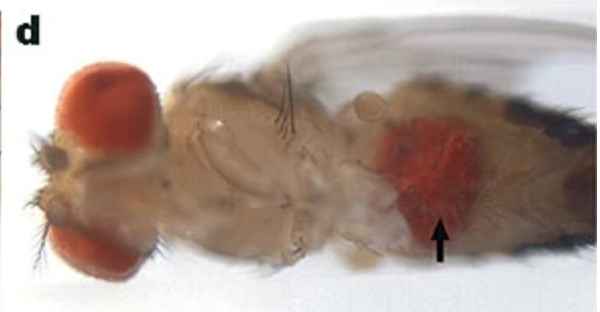
\includegraphics[width=0.7\textwidth]{image/eyeful_phenotype.png}
    \caption{Typical phenotype of $Eyeful$, from Ferres-Marco, D., Gutierrez-Garcia, I., Vallejo, D. et al. Epigenetic silencers and Notch collaborate to promote malignant tumours by Rb silencing. Nature 439, 430–436 (2006).}
    \label{eyeful_phenotype}
\end{figure}

According to Ferres et al., the eye tumours and metastases in the $Eyeful$ model are induced by two genes: \textit{psq} and \textit{lola}, together with the overexpression of \textit{Delta}. The mechanism behind eyeful and tumor metastases is that eyeful forces the transcription of two hitherto unsuspected growth and epigenetic genes, \textit{lola} and \textit{pipsqueak (psq)}, leading to changes of epigenetic pathways in growth control and tumorigenesis.\cite{ferres2006epigenetic}

The $Eyeful$ files we used in our experiments are constructed by Ferres et al. They used the Gene Search (GS) system to find genes that induces big eye phenotype with the overexpression of \textit{Delta}, and produced the $Eyeful$ line. 

The technique used to build the $Eyeful$ model is the gene search system, reported by Toba, G. et al.\cite{toba1999gene} The scheme of the technique is shown in the figure below.

\begin{figure}[H]
    \centering
    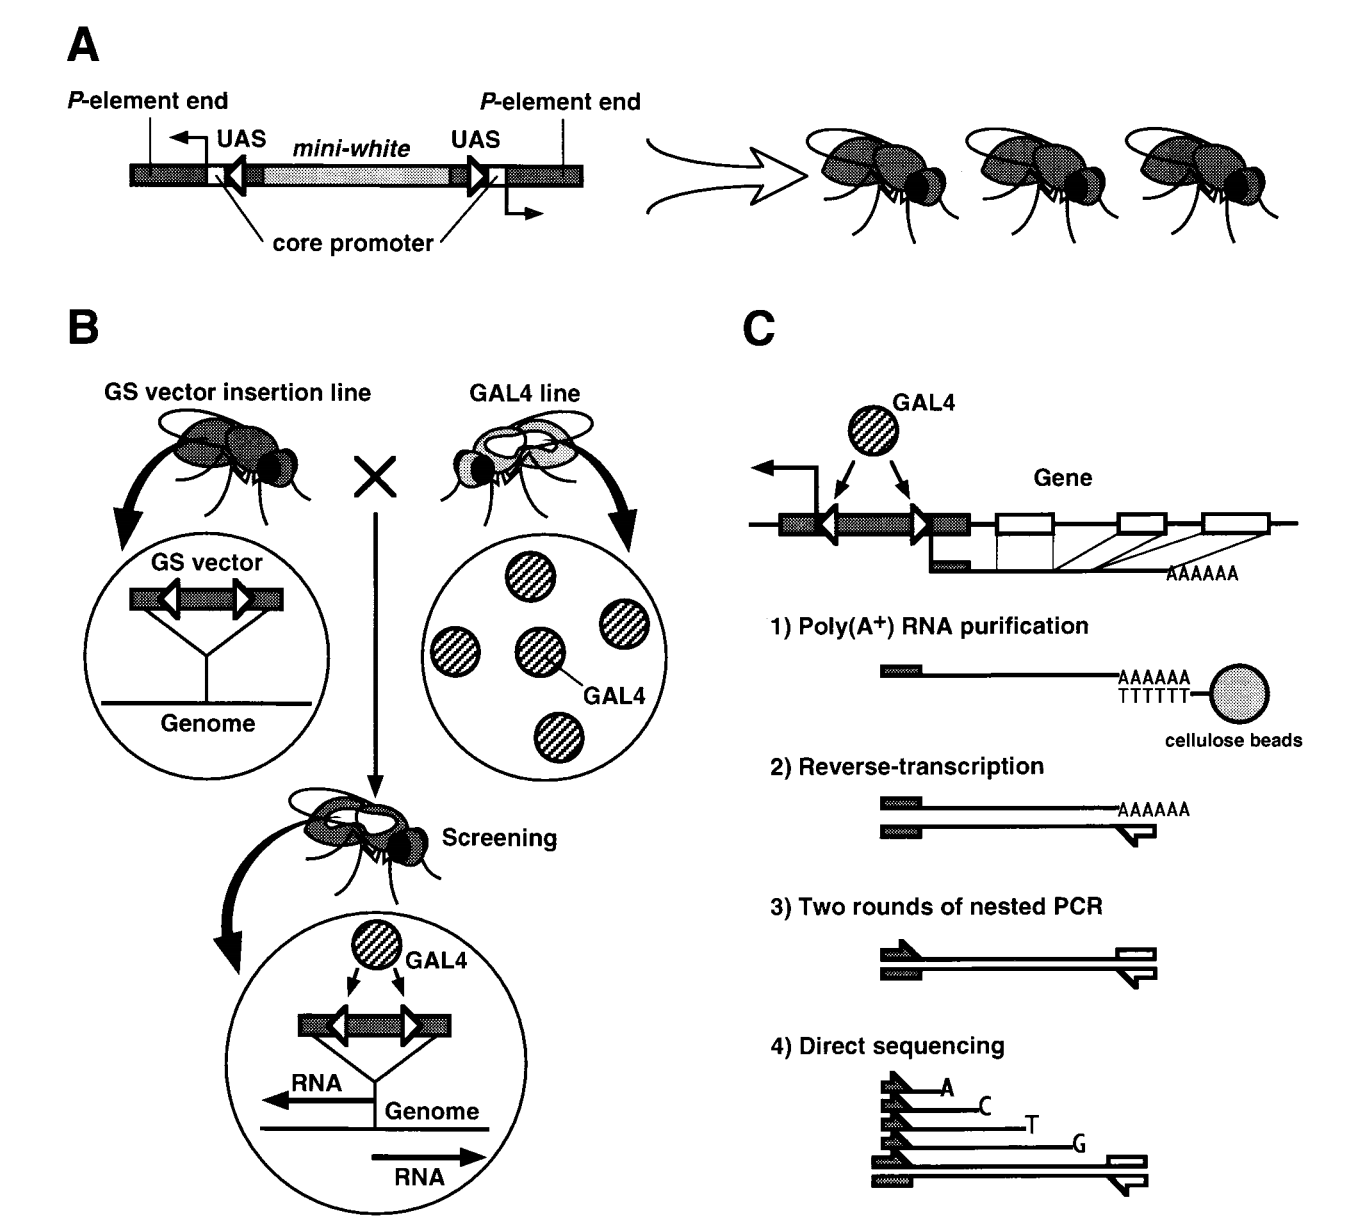
\includegraphics[width=0.7\textwidth]{image/gene_search.png}
    \caption{Schematic representation of the gene search system; by Toba, G. et al.}
    \label{eyeful_phenotype}
\end{figure}

In short, the gene search system involves the random insertion of a vector, which contains two copies of the upstream activating sequence (UAS) enhancer adjacent
to a core promoter, one copy near the terminal inverted repeats at each end of the vector, and oriented
to direct transcription outward. 

The vector is inserted to a $ey–Gal4 > Dl$ line (a triple mutant strain carrying the eyeful, UAS–Dl and ey–Gal4 transgenes all on the same chromosome) randomly, and the out-coming phenotype are screened.

\subsubsection{$Ras^{v12/Ig}$ model}
The $Ras^{v12/Ig}$ model consists of two lines:
\begin{enumerate}
    \item w;$Igl^4$ FRT40A UAS-$RAS^{v12}$/CyO;Sb/TM6B Tb
    \item yw ey-Flp; tub-Gal80 FRT40A; act>y+>Gal4 UAS-$GFP$
\end{enumerate}
The first line is used as the line to produce tumours and metastases in eye, brain and ventral nerve cord (VNC), while the second line with Gal4 is used to trigger the tumours and metastases in the former line, when the two lines are crossed.

Note that in the second line, ey-Flp is used. Flp-FRT recombination is a site-directed recombination technology, increasingly used to manipulate an organism's DNA under controlled conditions \textit{in vivo}. Different types of Flp-FRT recombination are briefly illustrated below.

\begin{figure}[H]
    \centering
    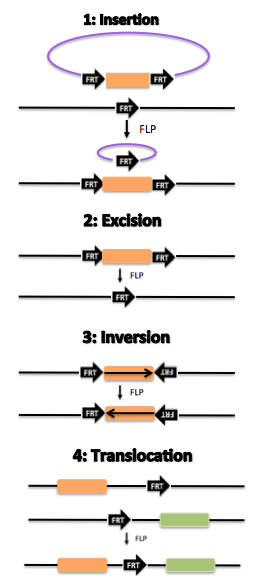
\includegraphics[width=0.25\textwidth]{image/Flp-FRT.png}
    \caption{Different types of Flp-FRT recombination}
    \label{Flp-FRT}
\end{figure}

The last type of Flp-FRT recombination explains how our model works. In \textit{Drosophila}, homozygous 
$Igl^4$ leads to lethal before larva of the 3rd instar, and therefore should be avoided in early stages of development. When the larva enters 3rd phase, ey-Flp can be properly expressed in the eye disc, leading to Flp-FRT recombination happen randomly during mitosis. The figure below shows how Flp-FRT recombination in our model.

\begin{figure}[H]
    \centering
    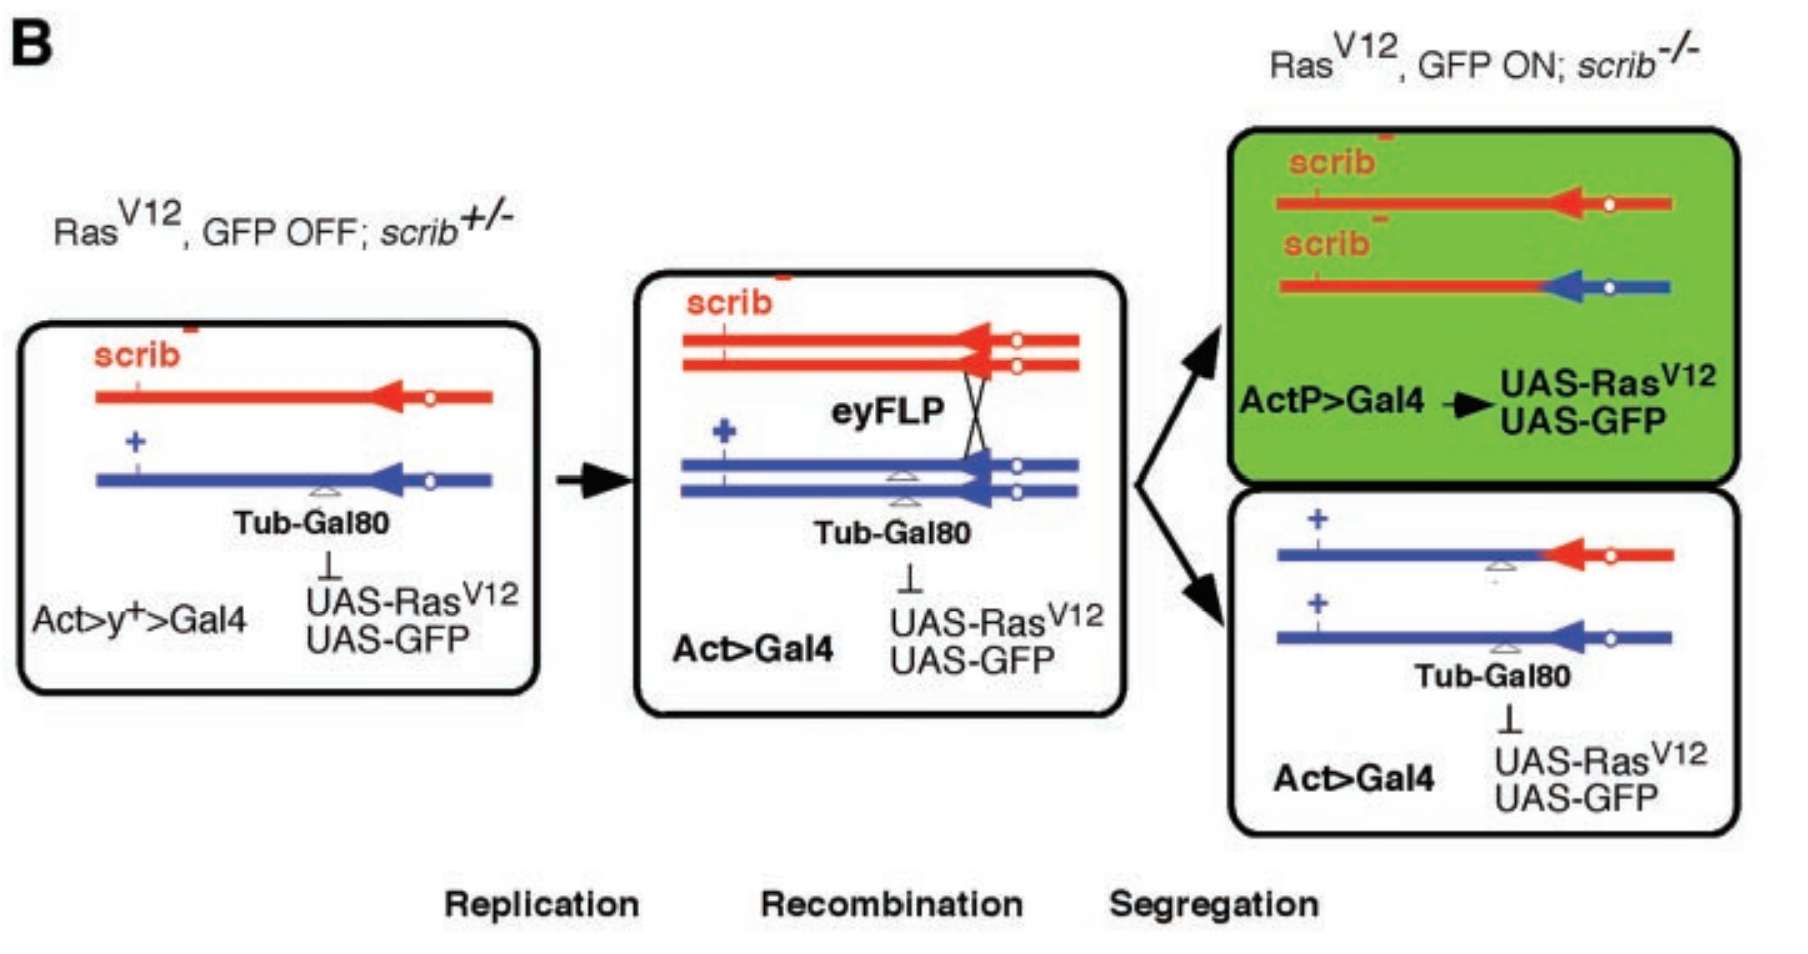
\includegraphics[width=0.7\textwidth]{image/FRT_RAS.png}
    \caption{How Flp-FRT recombination in our model; by Pagliarini, Raymond A and Xu, Tian}
    \label{FRT-RAS}
\end{figure}

Expression of the FLP recombinase in the developing eye ey-FLP mediates mitotic recombination between chromosome arms and produces clones of cells homozygously mutant for a gene that promotes metastatic behavior(i.e., scrib). Only these mutant cells lose the Gal80 repressor, which allows Gal4 of the eyFLP-activated Act>y>Gal4 “flip-out” construct to direct the constitutive expression of UAS-GFP and UAS-RasV12 (as well as othergenes of interest) regardless of their eventual locations and differentiation status. Gal80 expression in nonmutant cells also markedly reduces leaky flip-out construct expression in tissues outside of the eyeantennal region. Expression of GFP, RasV12, and other transgenes is therefore restricted to homozygous mutant cells. Multiple genetic alterations can be combined in the same cell and metastatic behavior can be monitored in vivo by following these GFP-expressing cells.\cite{pagliarini2003genetic}

Microinjection of the P-element plasmid which contains our target sequence into \textit{Drosophila} eggs is a common practise of building model files, and the P-element plasmid will be integrated to the genome. The files are then screened by their eye color, and crossed with tool files. Tool files are those files with double balancer chromosomes. After the crossing, desired chromosome will be identified and will become an allele chomosome with a balancer chromosome.
